\chapter{Process Interaction --- Mechanisms \& Problems}\label{chap:pi_process_interaction_mechanisms_problems} % (fold)
The algorithm for \hyperref[sec:cp_the_critical_section_problem]{The Critical Section Problem} described in the previous chapter can be run on a \textit{bare machine}.
They only use machine language instructions that the computer provides, too low level to be used efficiently and reliably.
\emptyln{}
Introduction of basic \textbf{mechanisms} and \textbf{abstractions} for \hyperref[def:process]{Process} coordination: provided directly by the \hyperref[def:conc-machine]{Concurrent Machine} and used in concurrent languages.
\begin{note}
    Main concepts:
    \begin{itemize}
        \item \textbf{semaphores};
        \item \textbf{monitors};
    \end{itemize}
\end{note}
%
\section{Semaphores}\label{sec:cp_semaphores} % (fold)
\begin{note}[Introduced by Dijkstra in 1968]
\end{note}
\begin{definition}{Semaphore}{semaphore}
    \textbf{Semaphores} are a very simple but powerful general-purpose construct which make it possible to solve almost any mutual exclusion and synchronization problems.
    Semaphore as a primitive data type provided by the \hyperref[def:conc-machine]{Concurrent Machine}
\end{definition}
\begin{quote}
    Informally, a semaphore functions as street semaphore, \textit{blocking} and \textit{unblocking} \hyperref[def:process]{Process} execution according to the need
\end{quote}
\paragraph{Semaphore Usage}\label{par:pi_semaphore_usage} % (fold)
Semaphores are \textbf{primitive constructs} that can be used as low-level building block to solve almost any problem concerning \hyperref[sub:cp_process_interaction]{Process Interaction} (in \textbf{shared memory} architecture).
\\
In particular, they can be used for both:
\begin{itemize}
    \item \textbf{mutual exclusion} (\hyperref[sec:cp_the_critical_section_problem]{Critical Section Problems}, \hyperref[sub:cp_locks]{Implementing Locks}, etc.);
    \item \textbf{synchronization} (event semaphore for signalling, barriers, etc.);
\end{itemize}
% paragraph Semaphore Usage (end)
%
\subsection{Semaphore Data Type}\label{sub:cp_semaphore_data_type} % (fold)
A semaphore $S$ is a compound data type with two fields:
\begin{itemize}
    \item $S.V$ is an integer $\ge 0$;
    \item $S.L$ is a \textbf{set} of \hyperref[def:process]{Process} id;
\end{itemize}
It can be initialized with
\begin{itemize}
    \item a value $k \ge 0$ for $S.V$
    \item the empty set $\pg{}$ for $S.L$
\end{itemize}
\begin{note}
    It provides two basic \textit{atomic} operations:
    \begin{itemize}
        \item \textbf{wait(S)}: also called $P(S)$ from Dijkstra original choice;
        \item \textbf{signal(S)}: also called $V(S)$ from Dijkstra original choice;
    \end{itemize}
\end{note}
%
\subsubsection{Wait Operation}\label{sub:pi_wait_operation} % (fold)
\begin{codeblock}{}
    wait(S) =
    < if (S.V > 0)
        S.V := S.V - 1
    else
        S.L := S.L = {p}
        p.state := blocked >
\end{codeblock}
\begin{description}
    \item[Description] If the value of the \hyperref[def:semaphore]{Semaphore} $V$ is $> 0$ (\textit{the semaphore is green}) then it is seimply decremented, otherwise if the value $V = 0$ (it the semaphore is red), then the process is blocked: $p$ is \textit{blocked on} the \hyperref[def:semaphore]{Semaphore} $S$
    \begin{note}[The \texttt{wait} is meant to be {\hyperref[def:atomic-object]{Atomic}}]
    \end{note}
\end{description}
% subsubsection Wait Operation (end)
%
\subsubsection{Signal Operation}\label{sub:pi_signal_operation} % (fold)
\begin{codeblock}{}
    signal(S) =
    < if (S.L = {})
        S.V := S.V + 1
    else
        let q := arbitrary element of S.L
        S.L := S.L - {q}
        q.state := ready >
\end{codeblock}
\begin{description}
    \item[Description] If no \hyperref[def:process]{Process} is waiting, then the semaphore value is incremented, otherwise select a \hyperref[def:process]{Process} $q$ \textbf{blocked} on the semaphore, and \textbf{unblock} it.
\end{description}
\begin{note}[Also \texttt{signal} is meant to be {\hyperref[def:atomic-object]{Atomic}}]
\end{note}
% subsubsection Signal Operation (end)
% subsection Semaphore Data Type (end)
%
\subsection{Semaphore Invariant}\label{sub:pi_semaphore_invariant} % (fold)
Let $k$ be the initial value of the integer component of the \hyperref[def:semaphore]{Semaphore}, \texttt{NUM(signal(S))} the number of \texttt{signal(S)} statements that \textbf{have been executed}, and \texttt{NUM(wait(S))} the number of \texttt{wait(S)} statements that \textbf{have been completely executed}.
\\
A \hyperref[def:process]{Process} that is blocked when executing \texttt{wait(S)} \textbf{is not considered} to have \textbf{successfully executed} the statement.
\begin{theorem}{Semaphore Invariant}{sema-inv}
    A \hyperref[def:semaphore]{Semaphore} $S$ satisfies the following invariants:
    \begin{codeblock}{}
    S.V >= 0
    S.V = l + NUM(signal(S)) - NUM(wait(S))
    \end{codeblock}
\end{theorem}
% subsection Semaphore Invariant (end)
%
\subsection{Type of Semaphores}\label{sub:pi_type_of_semaphores} % (fold)
\begin{description}
    \item[Mutex] Or \textit{binary semaphores} are \hyperref[def:semaphore]{Semaphores} whose integer component can take only two values: $0$ and $1$.
        \begin{note}
            The name derives from their typical use for implementing mutual exclusion
        \end{note}
    \item[General] Or \textit{counting} or \textit{resource semaphores} are \hyperref[def:semaphore]{Semaphores} whose integer component can take any value $\ge 0$.
    \item[Event] They are \hyperref[def:semaphore]{Semaphores} initialized with $0$ only used for \textbf{synchronization} purpose.
\end{description}
There are several different definitions of the \hyperref[def:semaphore]{Semaphore} type, differences relate to the specification of \hyperref[def:liveness-prop]{Liveness Properties}, and do not affect the \hyperref[def:safety-prop]{Safety Properties} that follow from the \hyperref[th:sema-inv]{Semaphore Invariant}.
\\
The main types are:
\begin{itemize}
    \item \textbf{strong} vs \textbf{weak} semaphores;
    \item \textbf{busy-wait} semaphores;
\end{itemize}
%
\subsubsection{Strong Semaphore}\label{sub:pi_strong_semaphore} % (fold)
In \textbf{strong} \hyperref[def:semaphore]{Semaphore} \texttt{S.L} is not a set, but a \textbf{queue}: 
\begin{note}[{\hyperref[def:semaphore]{Semaphores}} in which \texttt{S.L} is a set are called \textbf{weak}]
\end{note}
\begin{cimage}
    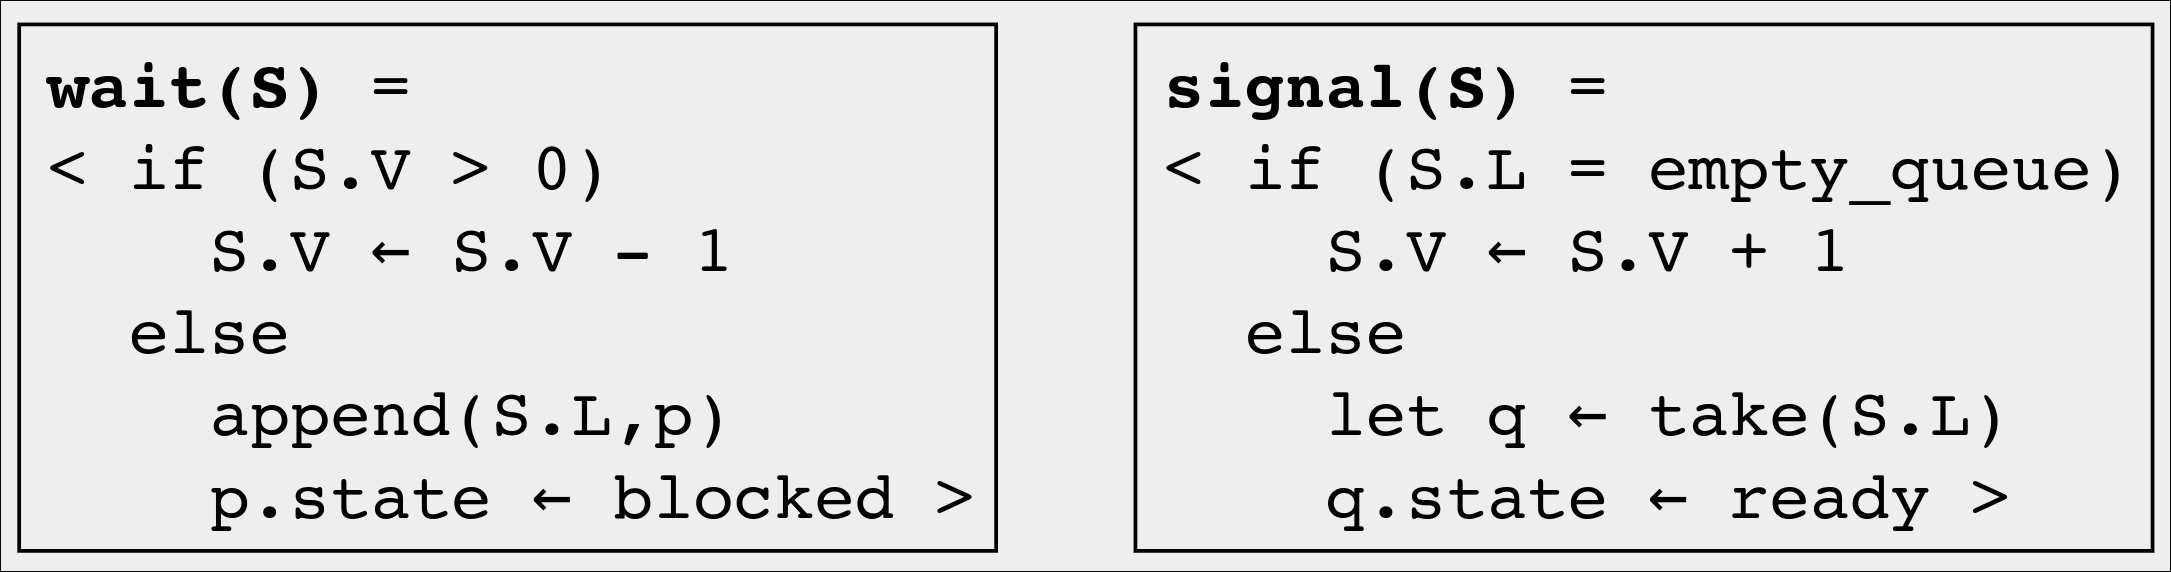
\includegraphics[width=.8\textwidth]{assets/20261019_201331.png}
\end{cimage}
\begin{warning}[Important property: no \red{starvation}]
    For a \red{strong semaphore} \hyperref[def:starvation]{Starvation} is impossible for any number $N$ of \hyperref[def:process]{Processes}
\end{warning}
% subsubsection Strong Semaphore (end)
%
\subsubsection{Busy-Wait Semaphore}\label{sub:pi_busy_wait_semaphore} % (fold)
They are \hyperref[def:semaphore]{Semaphores} without \texttt{S.L}: all operations are still \hyperref[def:atomic-object]{Atomic}, so there is no \hyperref[def:interleaving]{Interleaving} between two statements implementing the \hyperref[sub:pi_wait_operation]{Wait Operation}
\begin{cimage}
    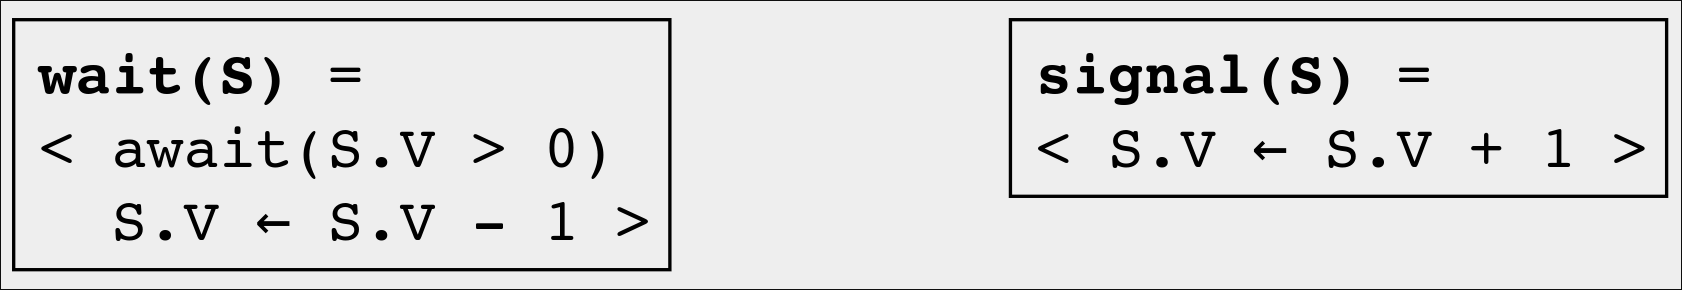
\includegraphics[width=.8\textwidth]{assets/20261019_201807.png}
\end{cimage}
\begin{warning}[Loosing freedom from {\hyperref[def:starvation]{Starvation}}]
    With \textbf{busy-wait semaphores} you cannot assume that a \hyperref[def:process]{Process} enters in its \hyperref[def:crit-sec]{Critical Section} event in the 2-process solution
\end{warning}
\begin{remark}{}{}
    Busy-wait semaphores are appropriate in a multiprocessor system when the waiting process has its own processor and is not wasting CPU time that could be used for computation.
    \begin{tip}
        They would be appropriate in a system with a little contention so that the waiting process would not waste too much CPU time
    \end{tip}
\end{remark}
% subsubsection Busy-Wait Semaphore (end)
% subsection Type of Semaphores (end)
%
\subsection{Critical Section With Semaphores}\label{sub:pi_critical_section_with_semaphores} % (fold)
Using a \hyperref[def:semaphore]{Semaphore}, the solution of \hyperref[sec:cp_the_critical_section_problem]{The Critical Section Problem} for two \hyperref[def:process]{Processes} is trivial.
\begin{note}[Using a semaphore as a lock]
\end{note}
\begin{ctable}{|l|l|}
    \hline
    \multicolumn{2}{|l|}{\textbf{CS with semaphores: 2 processes}} \\
    \hline
    \multicolumn{2}{|l|}{\texttt{binary semaphore $S\leftarrow\pt{1,\pg{}}$}} \\
    \hline
    \textbf{p} & \textbf{q} \\
    \hline
    \texttt{loop forever} & \texttt{loop forever} \\
    \textbf{p1:} \texttt{NCS} & \textbf{q1:} \texttt{NCS}  \\
    \textbf{p2:} \texttt{wait(S)} & \textbf{q2:} \texttt{wait(S)} \\
    \textbf{p3:} \texttt{CS} & \textbf{q3:} \texttt{CS} \\
    \textbf{p4:} \texttt{signal(S)} & \textbf{q4:} \texttt{signal(S)} \\
    \hline
\end{ctable}
\begin{outerproof}{Proving Correctness}{}
    Building the reduced \hyperref[def:state-diagram]{State Diagram} and checking properties:
    \begin{ctable}{|l|l|}
        \hline
        \multicolumn{2}{|l|}{\textbf{CS with semaphores: 2 processes (abbreviated)}} \\
        \hline
        \multicolumn{2}{|l|}{\texttt{binary semaphore $S\leftarrow\pt{1,\pg{}}$}} \\
        \hline
        \textbf{p} & \textbf{q} \\
        \hline
        \texttt{loop forever} & \texttt{loop forever} \\
        \textbf{p1:} \texttt{wait(S)} & \textbf{q1:} \texttt{wait(S)} \\
        \textbf{p2:} \texttt{signal(S)} & \textbf{q2:} \texttt{signal(S)} \\
        \hline
    \end{ctable}
    It can be verified that the \hyperref[def:semaphore]{Semaphore} solution for \hyperref[sec:cp_the_critical_section_problem]{The Critical Section Problem} is correct: there is \textbf{mutual exclusion}, \textbf{free from \hyperref[def:deadlock]{Deadlock}} and \hyperref[def:starvation]{Starvation}.
\end{outerproof}
\begin{remark}{The \hyperref[def:state-diagram]{State Diagram}}{}
    \begin{itemize}
        \item \hyperref[def:semaphore]{Semaphore} structure in the tuple \hyperref[def:state]{State} \texttt{\{s.V, s.L\}}
        \item \textbf{Blocked} \hyperref[def:state]{State} for $P$ and $Q$ is labelled as \texttt{p1B} and \texttt{q1B}
    \end{itemize}
    \begin{cimage}
        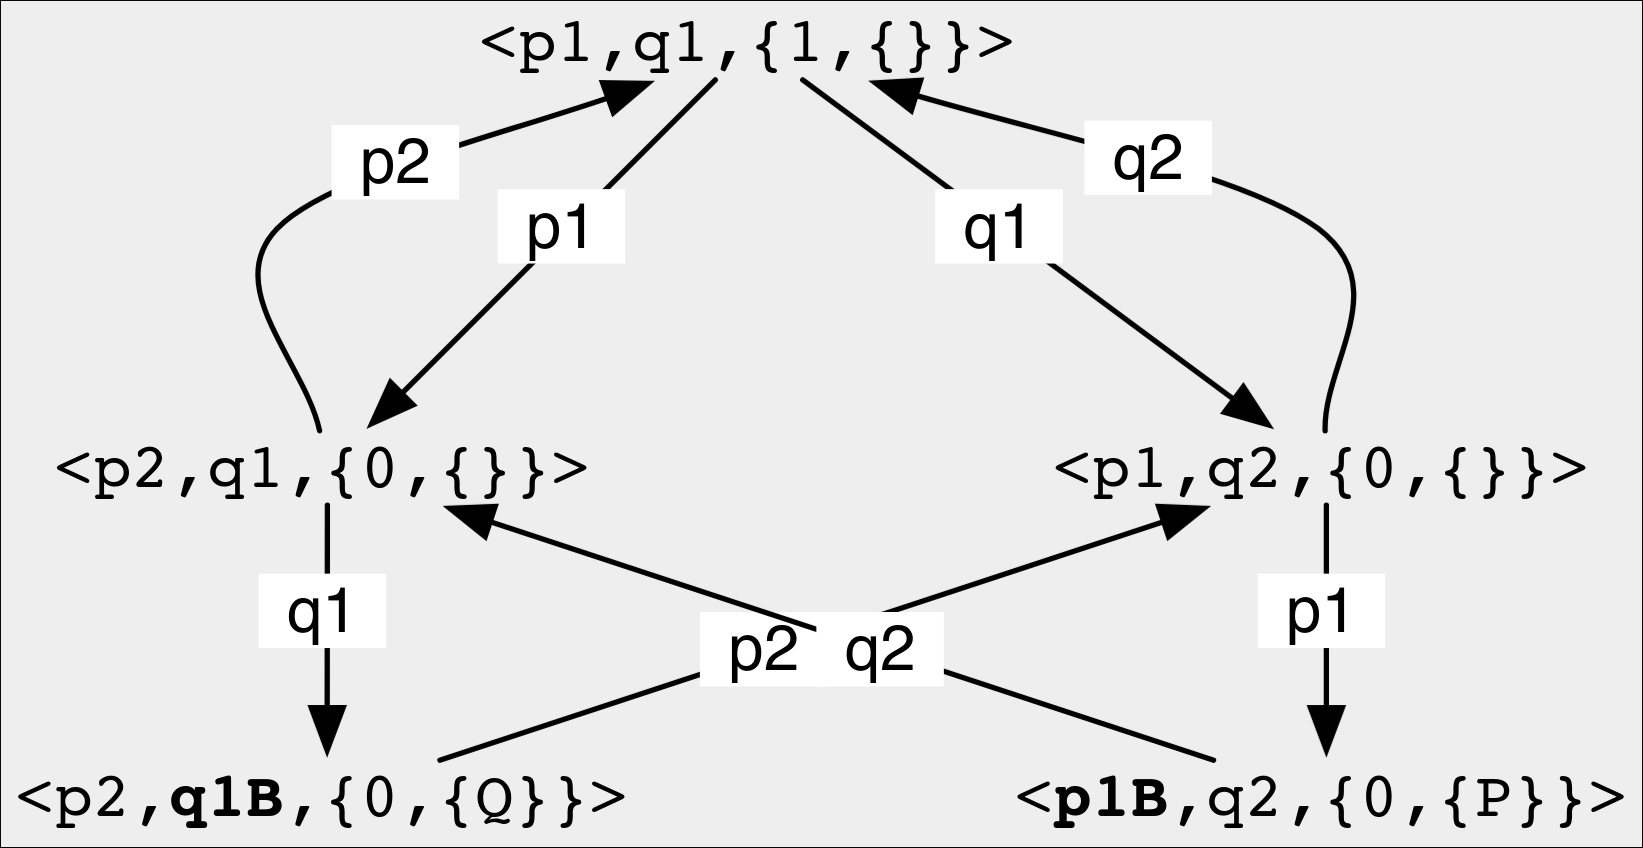
\includegraphics[width=.6\textwidth]{assets/20261019_203149.png}
    \end{cimage}
\end{remark}
%
% subsection Critical Section With Semaphores (end)
%
\subsection{Critical Section for $N$ Processes}\label{sub:pi_critical_section_for_n_processes} % (fold)

% subsection Critical Section for $N$ Processes (end)
% section Semaphores (end)
% chapter Process Interaction --- Mechanisms \& Problems (end)
